\documentclass[12pt]{article}
\usepackage{latexsym}
\usepackage{epsfig}
\usepackage{amsmath}
\usepackage{amssymb}
\usepackage{tikz} 

\setlength{\topmargin}{0in}
\setlength{\leftmargin}{0in}
\setlength{\textwidth}{6in}
\setlength{\textheight}{9.5in}
\setlength{\parindent}{0.2in}
\setlength{\parskip}{.08in}
\voffset = -.45in
\hoffset = -.5in
\def\filledbox{\vrule height 1.8ex width .8ex depth -.1ex } % square bullet
\newcommand{\qed}{\large ~$\Box$ \normalsize}
%
%\newtheorem{thm}{Theorem}
%\newenvironment{theorem}{\begin{thm}\ \rm}{\end{thm}}
%
%\newtheorem{lem}{Lemma}
%\newenvironment{lemma}{\begin{lem}\ \rm}{\end{lem}}
%
\newtheorem{theorem}{Theorem}
\newtheorem{lemma}{Lemma}
\newtheorem{corollary}{Corollary}
\newenvironment{proof}{{\noindent \bf Proof\ \ }}{\qed}
\newenvironment{proofsketch}{{\noindent {\bf Proof}\ (sketch)\ \ }}{\qed}
%
\def\shh{\skew3\hat{\hat s}}
\def\dhh{\skew6\hat{\hat d}}
\begin{document}
\newcommand{\I}{\mbox{{\em Int}}}
\newcommand{\lt}{\mbox{{\em left}}}
\newcommand{\rt}{\mbox{{\em right}}}
\newcommand{\ld}{\Delta^l}
\newcommand{\rd}{\Delta^r}
\newcommand{\lsp}[1]{\large\renewcommand{\baselinestretch}{#1}\normalsize}
\newcommand{\hsp}{\hspace{.2in}}

\def\Endwhile{\mbox{\bf endwhile\ }}
\def\Or{\mbox{\bf or\ }}
\def\Do{\mbox{\bf do\ }}
\def\Downto{\mbox{\bf downto\ }}
\def\Int{\mbox{\bf int\ }}
\def\To{\mbox{\bf to\ }}
\def\Repeat{\mbox{\bf repeat\ }}
\def\Until{\mbox{\bf until\ }}
\def\Return{\mbox{\bf return\ }}
\def\Not{\mbox{\bf not\ }}
\def\And{\mbox{\bf and\ }}
\def\For{\mbox{\bf for\ }}
\def\Foreach{\mbox{\bf foreach\ }}
\def\Else{\mbox{\bf else\ }}
\def\Elseif{\mbox{\bf elseif\ }}
\def\End{\mbox{\bf end\ }}
\def\If{\mbox{\bf if\ }}
\def\Mod{\mbox{\bf \ mod\ }}
\def\Then{\mbox{\bf then\ }}
\def\While{\mbox{\bf while\ }}
\def\Output{\mbox{\bf output\ }}


\lsp{1}
\pagestyle{plain}
\begin{center}
{\bf
DFS Worksheet
}
\end{center}

\begin{figure}[h]
\center{}
\includegraphics[width = 3in]{DFS.pdf}
\end{figure}

\begin{enumerate}
\item Label each vertex with its discovery and finish time stamp.

\begin{center}
    \begin{tabular}{|c|c|c|}
     \hline \textbf{Vertex} & \textbf{d} & \textbf{f} \\
     \hline a & 1 & 10 \\
     \hline b & 11 & 16 \\
     \hline c & 12 & 15 \\
     \hline d & 13 & 14 \\
     \hline e & 2 & 9 \\
     \hline f & 3 & 8 \\
     \hline g & 5 & 6 \\
     \hline h & 4 & 7 \\
     \hline
    \end{tabular}
\end{center}

\item Draw the depth-first tree. (Augment with back, cross and forward edges.)

\begin{center}
    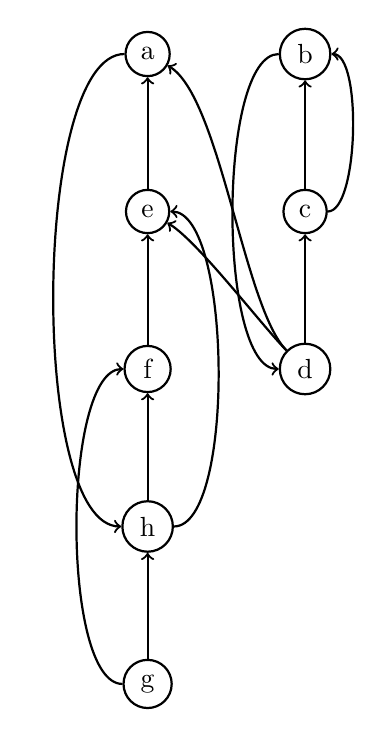
\begin{tikzpicture}[node distance={2cm}, thick, main/.style = {draw, circle}] 
        \node[main] (1) {a};
        \node[main] (2) [right of=1] {b};
        \node[main] (3) [below of=2] {c};
        \node[main] (4) [below of=3] {d};
        \node[main] (5) [below of=1] {e};
        \node[main] (6) [below of=5] {f};
        \node[main] (8) [below of=6] {h};
        \node[main] (7) [below of=8] {g};

        % tree edges
        \draw[->] (5) -- (1); 
        \draw[->] (6) -- (5); 
        \draw[->] (8) -- (6); 
        \draw[->] (7) -- (8);
        \draw[->] (4) -- (3);
        \draw[->] (3) -- (2);

        % back edges
        \draw[->] (7) to [out=180,in=180,looseness=.5] (6); 
        \draw[->] (8) to [out=0,in=0,looseness=.5] (5); 
        \draw[->] (3) to [out=0,in=0,looseness=.5] (2); 

        % forward edges
        \draw[->] (1) to [out=180,in=180,looseness=.5] (8); 
        \draw[->] (2) to [out=180,in=180,looseness=.5] (4); 

        % cross edges
        \draw[->] (4) to [out=135,in=330,looseness=.5] (1); 
        \draw[->] (4) to [out=135,in=330,looseness=.5] (5); 
        
        % \draw (1) to [out=180,in=270,looseness=5] (1); 
        % \draw (2) -- (4); 
        % \draw (3) -- (4); 
        % \draw (5) -- (4); 
        % \draw[->] (5) to [out=315, in=315, looseness=2.5] (3);  
    \end{tikzpicture}
\end{center}

\pagebreak
\item Show the discovery-finish range for vertices $a$, $f$ and
$b$ on a number-line. \\ I am not sure why the graph is above it and I can't fix it in latex sorry.


\begin{figure}
    \includegraphics[width = 6in]{numberline.jpg}
\end{figure}
\end{enumerate}
\end{document}
